\documentclass[border=10pt]{standalone}
\usepackage{tikz}
\usetikzlibrary{arrows.meta}

\begin{document}
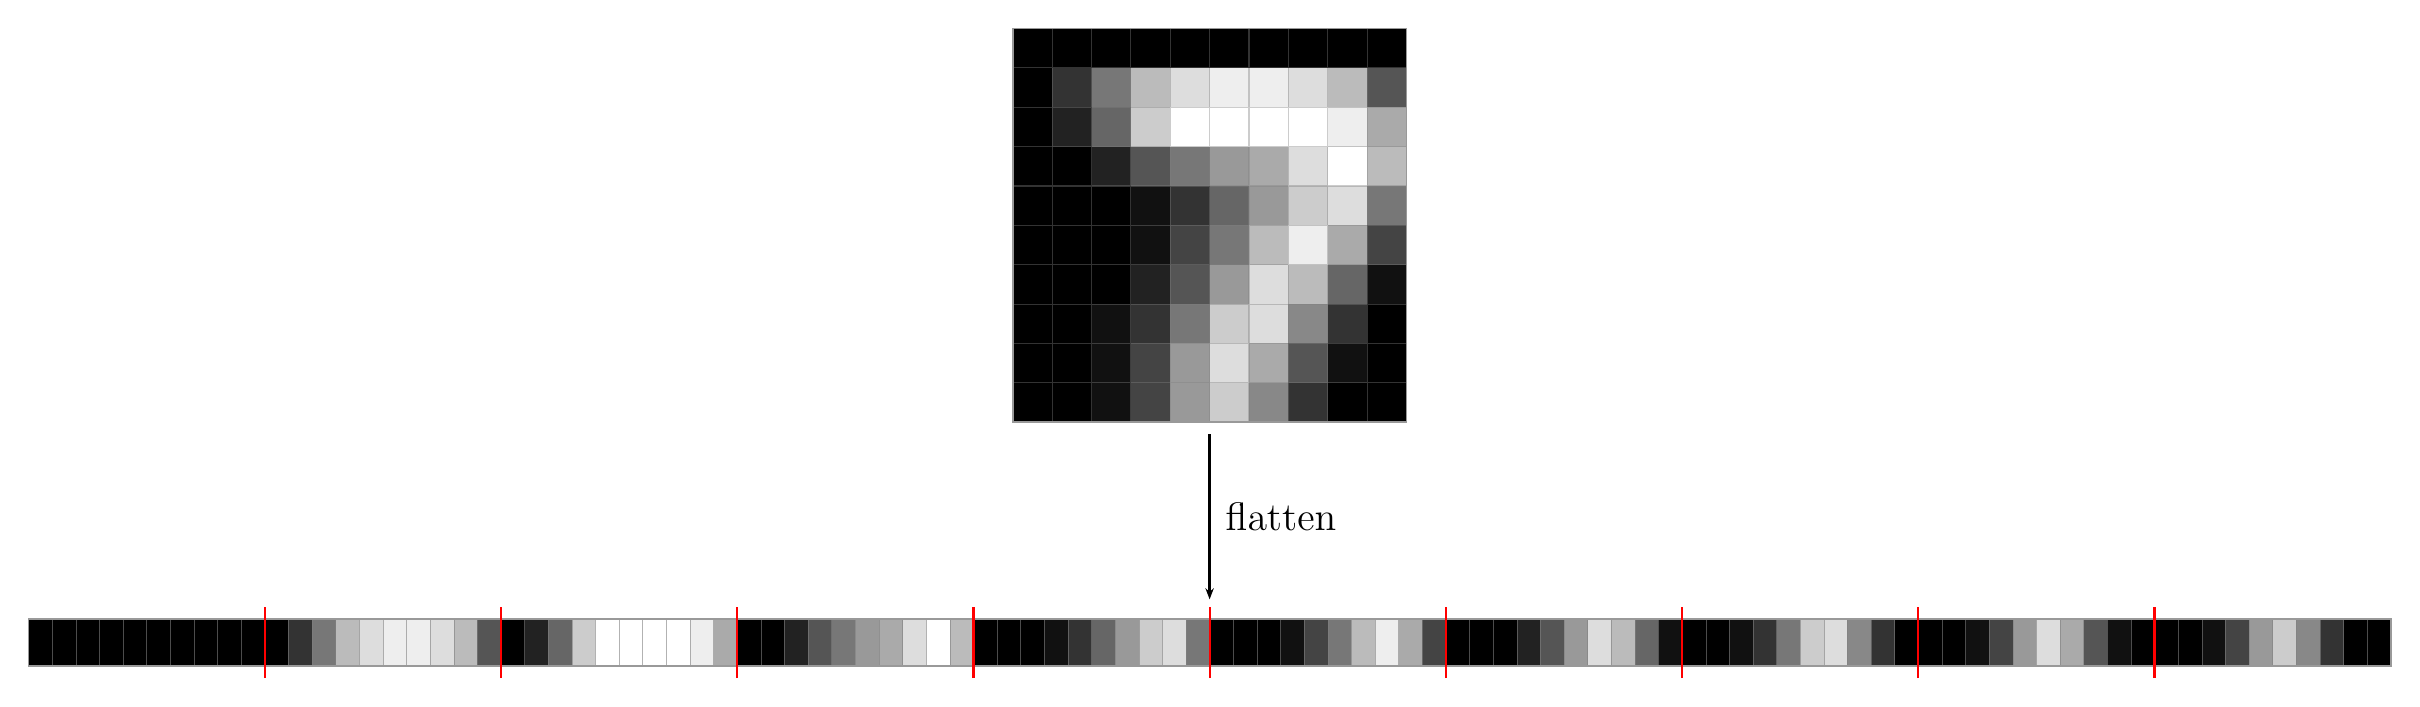
\begin{tikzpicture}[>={Stealth[length=4pt]}, line width=0.8pt, font=\large]

  % ---------- 黑底：10x10 图（格 0.5cm，左下角 (12.5,3)） ----------
  \fill[black] (12.5,3) rectangle (17.5,8);

  % ---------- 一次循环同时画：10x10 图 + 展开的 100 格 ----------
  \foreach \v [count=\n] in {%
    0,0,0,0,0,0,0,0,0,0,%                                    行1
    0,3,7,11,13,14,14,13,11,5,%                              行2
    0,2,6,12,15,15,15,15,14,10,%                             行3
    0,0,2,5,7,9,10,13,15,11,%                                行4
    0,0,0,1,3,6,9,12,13,7,%                                  行5
    0,0,0,1,4,7,11,14,10,4,%                                 行6
    0,0,0,2,5,9,13,11,6,1,%                                  行7
    0,0,1,3,7,12,13,8,3,0,%                                  行8
    0,0,1,4,9,13,10,5,1,0,%                                  行9
    0,0,1,4,9,12,8,3,0,0 %                                   行10
  }{%
    \pgfmathtruncatemacro{\col}{int(mod(\n-1,10))}
    \pgfmathtruncatemacro{\row}{int((\n-1)/10)}
    \pgfmathsetmacro{\gpct}{\v/15}
    \definecolor{px}{gray}{\gpct}
    % 10x10 图的像素
    \fill[px] ({12.5+0.5*\col}, {3+0.5*(9-\row)}) rectangle ++(0.5,0.5);
    % 展开条的第 n 格（0.3 x 0.6，紧紧挨在一起；整体上移 0.5）
    \fill[px] ({0.3*(\n-1)}, -0.1) rectangle ++(0.3,0.6);
  }

  % ---------- 10x10 图的网格与边框 ----------
  \draw[gray, opacity=0.4, thin, step=0.5] (12.5,3) grid (17.5,8);
  \draw[gray!80, line width=0.6pt] (12.5,3) rectangle (17.5,8);

  % ---------- 展开条：细格线 + 外边框 ----------
  \foreach \k in {1,...,99}
    \draw[gray, line width=0.15pt, opacity=0.6] ({0.3*\k},-0.1) -- ({0.3*\k},0.5);
  \draw[gray!80, line width=0.6pt] (0,-0.1) rectangle (30,0.5);

  % ---------- 每 10 格一条红线 ----------
  \foreach \k in {1,...,9}
    \draw[red, line width=0.8pt] ({3*\k},-0.25) -- ({3*\k},0.65);

  % ---------- flatten 箭头（字放大，箭头缩短贴近展开条） ----------
  \draw[->, line width=1pt] (15,2.85) -- (15,0.75)
    node[midway, right=2pt, font=\Large] {flatten};

  % ---------- 文字 ----------
%   \node[font=\large] at (15,8.7)  {$10\times10$ image};
%   \node[font=\large] at (15,-1.8) {flattened vector ($100$)};
%   \node[font=\tiny] at (0.15,-1.05)  {1};
%   \node[font=\tiny] at (2.85,-1.05)  {10};
%   \node[font=\tiny] at (27.15,-1.05) {91};
%   \node[font=\tiny] at (29.85,-1.05) {100};
\end{tikzpicture}
\end{document}